

En la figura (\ref{fig:aciertos-vs-k}), se muestra la cantidad de aciertos obtenidos para distintos k (componentes principales). 
Cada curva representa el delta utilizado en el criterio de parada.


\begin{figure}[h]
\begin{center}
  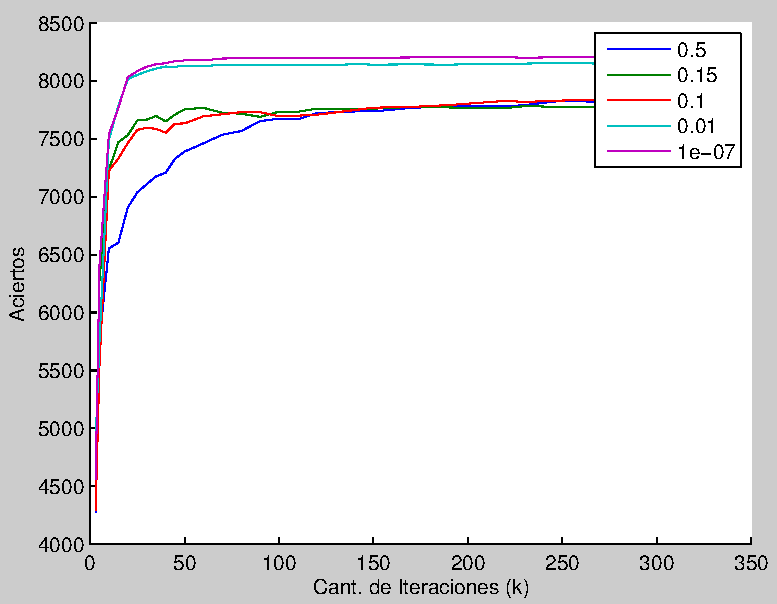
\includegraphics[scale=0.8]{imagenes/aciertos.pdf}
\end{center}
\caption{Gráfico de aciertos vs cantidad de iteraciones.}
\label{fig:aciertos-vs-k}
\end{figure}

En la figura (\ref{fig:tiempo-vs-k}), se muestra el tiempo de la ejecución del programa son contar el tiempo que tarda en
cargar la matriz de covarianza, para distintos valores de delta.

\begin{figure}[h]
\begin{center}
  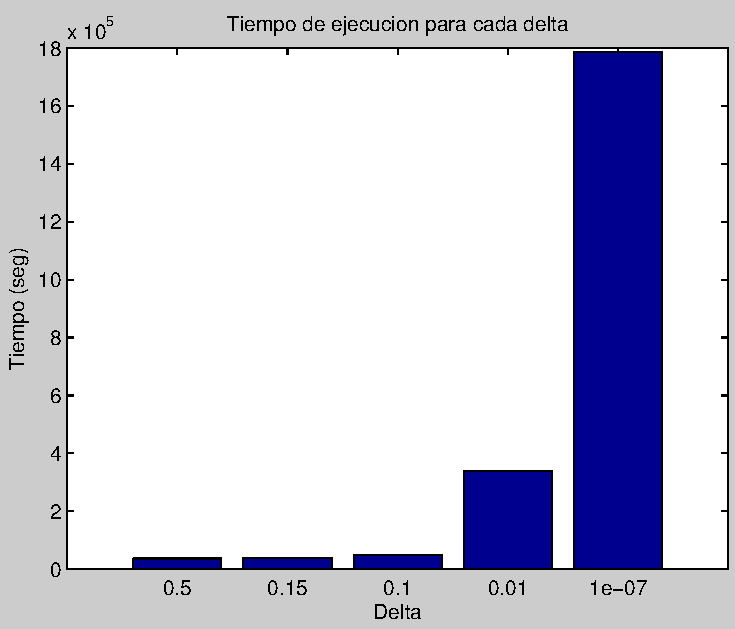
\includegraphics[scale=0.8]{imagenes/tiempos.pdf}
\end{center}
\caption{Gráfico de tiempo de ejecución vs delta.}
\label{fig:tiempo-vs-k}
\end{figure}